\documentclass[addpoints, 12pt]{exam}
\usepackage[utf8]{inputenc}
\usepackage{amsmath,amsthm,amsfonts,amssymb,amscd}
\usepackage{multirow,booktabs}
\usepackage[table]{xcolor}
\usepackage{fullpage}
\usepackage{lastpage}
\usepackage{enumitem}
% \usepackage{fancyhdr}
\usepackage{mathrsfs}
\usepackage{wrapfig}
\usepackage{setspace}
\usepackage{multicol}
\usepackage[retainorgcmds]{IEEEtrantools}
\usepackage[margin=3cm]{geometry}
\usepackage{listings}
\usepackage{pgf}
\usepackage{pgfplots}
\pgfplotsset{soldot/.style={color=red,only marks,mark=*, mark options={scale=1.5}},
             holdot/.style={color=red,fill=white,only marks,mark=*, mark options={scale=1.5}},
             compat=1.12}
\usepgfplotslibrary{external}
\usepgfplotslibrary{fillbetween}
\usetikzlibrary{intersections, calc, angles, quotes}
\usepackage{floatrow}
\newlength{\tabcont}
\setlength{\parindent}{0.0in}
\setlength{\parskip}{0.05in}
\newcommand\assignment{Week 1 Practice Problems}
\newcommand\school{SouthLake Christian Academy}
\newcommand\course{AP CSP}
\newcommand\examdate{August 2022}

\newcommand*{\texthide}[1]{\underline{\phantom{#1}}}
\newcommand*{\textshow}[1]{\underline{#1}}

\lstdefinestyle{mystyle}{
    basicstyle=\ttfamily\footnotesize,
    breakatwhitespace=false,         
    breaklines=true,                 
    captionpos=b,                    
    keepspaces=true,                 
    numbers=left,                    
    numbersep=5pt,                  
    showspaces=false,                
    showstringspaces=false,
    showtabs=false,                  
    tabsize=2
}
\lstset{style=mystyle}

\pagestyle{head}
\firstpageheader{Name: \\ Section: }{\textbf{\Large \assignment}}{Date: \hspace{5em}}%
\firstpageheadrule

\begin{document}

\begin{center}\textit{Feel free to use the paper tool we made in class!}\end{center}

\begin{questions}
		
	\question Recall that we looked at ASCII in lecture, which uses just 7 or 8 bits to represent letters of the alphabet.

    \begin{parts}
        \part Read up on ``Unicode", via Google, and explain in your own words how Unicode is able to represent many more symbols than can ASCII,
        which is particularly helpful for written languages with many more characters than English.
        \vfill
        \part What is the binary number that corresponds to the Unicode character ``A"?
        \vfill
    \end{parts}

	\question Decode the message:
    
    \texttt{0b01000001 01101110 01110011 01110111 01100101 01110010 00100000 01101001 01110011 00100000 00110100 00110010 00101110}
    \vfill

    \newpage

    \question ``Digitize'' the following audio (analog) signal by choosing a sampling frequency,
    drawing ``lollipops'' at that sampling frequency,
    and recording the approximate amplitude of each ``lollipops''. Use as many rows of the chart as needed!

    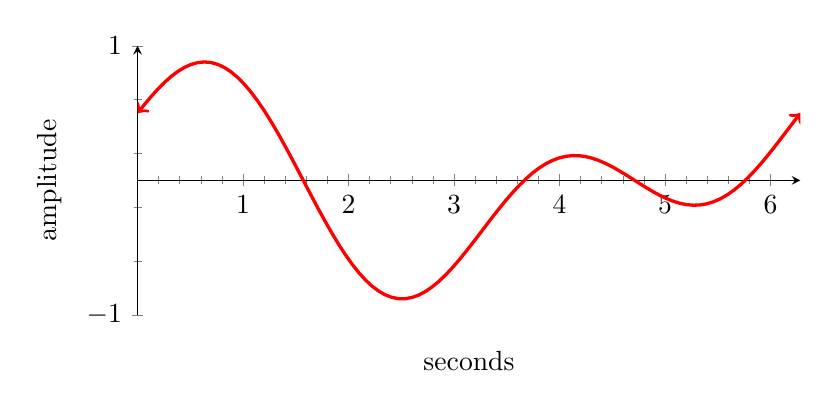
\begin{tikzpicture}
        \begin{axis}[
            axis lines = middle,
            xmin = 0, xmax = 2*pi,
            ymin = -1, ymax = 1,
            width=10cm, height=5cm,
			domain=0:2*pi,
            minor y tick num=4,
            minor x tick num=4,
            x label style={at={(axis description cs:0.5,-0.1)},anchor=north},
            y label style={at={(axis description cs:-0.1,.5)},rotate=90,anchor=south},
            xlabel={seconds},
            ylabel={amplitude},
			ytick={-1, 1},
			yticklabels={$-1$, $1$}
        ]
		
			\addplot[color=red, very thick, <->,domain=0:2*pi, samples=100] (x, {0.5*sin(deg(2*x)) + 0.5*cos(deg(x))});

        \end{axis}
    \end{tikzpicture}

    \begin{table}[h]
        \begin{tabular}{|c|c|}
        \hline
        Time (seconds) & Amplitude/Volume \\
        \hline
                       &                  \\
        \hline
                       &                  \\
        \hline
                       &                  \\
        \hline
                       &                  \\
                       \hline
                       &                  \\
                       \hline                      
                       &                  \\
                       \hline
                       &                  \\
                       \hline
                       &                  \\
                       \hline
                       &                  \\
                       \hline
                       & \\
                       \hline            
        \end{tabular}
    \end{table}

    \question If an image originally takes up 20kb of memory,
    and a certain algorithm compresses that image down to 10kb,
    what is the compression rate of this algorithm?
    \vfill

    

\end{questions}

\end{document}